\section{Каноническая схема генетического алгоритма.}

Генетические алгоритмы используют мутации и скрещивания. Чаще всего применяются к задачам, заданным на строках фиксированной длины над фиксированным алгоритмом. 

Каноническая схема генетического алгоритма:


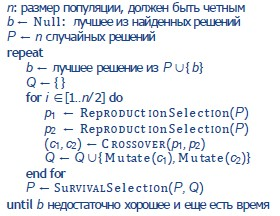
\includegraphics[width=8cm]{images/13bilet.jpg}  



Заметим, что мы получаем из 2 родителей 2 детей. Это происходит для того, чтобы сохранить все гены.